\documentclass[11pt, oneside]{article}   	% use "amsart" instead of "article" for AMSLaTeX format
\usepackage{geometry}                		% See geometry.pdf to learn the layout options. There are lots.
\geometry{a4paper}                   		% ... or a4paper or a5paper or ... 
\geometry{legalpaper, portrait, margin=1in}
\widowpenalty=500
\usepackage[parfill]{parskip}    			% Activate to begin paragraphs with an empty line rather than an indent
\usepackage{graphicx}				% Use pdf, png, jpg, or eps§ with pdflatex; use eps in DVI mode
\usepackage{amssymb}
\usepackage{multicol}
\usepackage{abstract} 
\usepackage{graphicx}
\usepackage{caption}

\title{Saito Consensus: Fixing the Market Failures in Bitcoin }
\author{David Lancashire, Richard Parris }
\date{December 24, 2020\\v. 4.0.1}
\begin{document}
\maketitle


\begin{onecolabstract}
Saito fixes the collective action problems that impede scaling in proof-of-work and proof-of-stake blockchains by coupling a circular ledger to a consensus mechanism that incentivizes the collection and sharing of transaction fees. The resulting network pays not just for mining and staking, but for all activities that contribute economic value to the network. In the process Saito fully eliminates majoritarian among other attacks.
\end{onecolabstract}

\begin{multicols}{2}
Saito pays user-facing infrastructure nodes out of an open consensus mechanism. Because this approach scales naturally, it incentivizes the processing of large amounts of data and can be used to build decentralized versions of many data-heavy services, such as un-astroturfable data exchanges, authentication and monetization applications, distributed key registries that are secure from MITM attacks, payment channels, and much more.

In economic terms, Saito can be understood as a solution for inducing a free market to deliver a public good. The design corrects the collective action problems inherent in the proof-of-work and proof-of-stake mechanisms, so that profit-seeking actors compete to bring money into the network, permitting scalability to the point that underlying network hardware rather than economic constraints impose limits on blockchain growth. We believe the practical limit for a Saito blockchain today is in the order of 100 TB of data per day, and advances in routing capacity will push us to the petabyte level within a decade.

The next section describes briefly the economic problems that need to be solved in order to build a scalable blockchain. The following sections outlines how Saito solves these problems and describes an implementation of these methods.


1. THE PROBLEM

The problem with blockchain scaling is not at the network technology layer: at the time of writing, data centers around the world are implementing 400 Gbps network switches while 100 Gbps connections are becoming standard even in lower-tier colocation facilities. If we had the resources to pay for the necessary equipment there is nothing technically stopping us from building a blockchain that is as decentralized and open as the public Internet backbone.

What limits network growth is the challenge of paying for the network. In the past, non-economists have waved away this limitation, claiming that as long as {\textit{someone}} is earning money from the network they will pay all costs necessary to support it. But this is not true, for proof-of-work and proof-of-stake networks are afflicted by two market failures:  a tragedy-of-the-commons problem that leads to blockchain bloat and eventual collapse and a free-rider problem that leads to an under-provision of user-facing network infrastructure and an over-provision of paid activities like mining and staking. Neither problem is crippling at small scale, but they grow incapacitating as bandwidth and storage costs rise.

Are there alternatives? Faced with the need to pay for uncompensated network infrastructure, computer scientists throw the problem to the market. As economists have known since the 1960s, asking the private sector to fund non-excludable infrastructure requires closure somewhere in the economic model. Businesses that pay for fee collection must necessarily close access to the fees they receive. The controlled flow of funds into the blockchain then undermines the openness of the  consensus layer. 

The only viable solution is to eliminate these market failures on the incentive level. Before the solution can be understood, it must be seen clearly. The major issues are as follows.

The tragedy-of-the-commons issue is created by the existence of the permanent ledger, which encourages nodes to accept payment today for work that can be offloaded to others tomorrow.  This incentive leads to bloated blockchains and more subtly to transaction mis-pricing, as users can pay fees that do not reflect the true cost of their transaction to the overall network. The fact that this is a fundamental problem is self-evident from the way Satoshi’s solution is ”not to care,” an approach that stops being viable in networks that operate at serious economic scale.

Eliminating the tragedy-of-the-commons problem requires all nodes that add transactions to the blockchain bear the cost of processing those transactions for as long as they remain on the blockchain. In practice, this requires a market mechanism for accurately determining the price of on-chain data storage. It also requires eliminating blockchain creep or deferring fee collection so that payments are meted-out over time as the node continues to do the work required for payment. Our solution to this problem is described in Section 2.

The free-rider problem is more insidious. It arises in blockchains where payments are made for one specific type of work (such as mining or staking) at the expense of other necessary activities. This mismatch incentivizes participants to maximize their spending on paid work and minimize spending on anything else. In the blockchain space, this results in miners and stakers "free-riding" on those who do the unpaid work of collecting fees or developing applications or otherwise supporting the user-facing network. The problem gets worse as the network scales, and evolutionary pressures make the trap inescapable: any Bitcoin miner that spends a smaller percent of its revenue on hashing than its more altruistic peers will lose market share until it also capitulates.

In economics, the typical solution to the free-rider problem is to eliminate the property of "non-excludability" associated with any good or service: restricting its benefits to those who pay the costs of provision. In the blockchain space this is impossible to do without destroying the openness of the network. Computer scientists often address the problem by adding protective middleware, such as wrapping consensus payments in closed voting rings which are of course themselves susceptible to these attacks. The jiggery-pokery can never these economic problem: markets are powerful enough to undermine these structures exactly because they incentivize it.

Without a solution to this problem our choice is between a network that cannot scale because it cannot pay for network operations, or a network that scales but loses the openness, trustlessness and economic self-sufficiency that makes the blockchain a useful invention. Neither approach is useful for building a genuinely open blockchain at massive scale.

The theoretical solution to the free-rider problem requires eliminating the possibility of free-riding: fixing the underlying incentive structure so that participants are paid for providing what the network actually needs. Because the blockchain requires a quantifiable cost-of-attack, this requires eliminating "mining" and "staking" and shifting to a different form of work that measures and pays nodes in proportion to the "value" they provide the network instead of the amount of hashing or staking they do.

This requires us to find a new way to measure value and then pay nodes in proportion to the amount of it they contribute. Accomplishing this requires deriving our measure of "work" from the transaction fees that users pay. The work of routing transaction fees into the network is the work that our network must encourage. Honest nodes can be induced to do this work by a share of the fees collected. The difficulty shifts to ensuring this mechanism preserves the cost-of-attack properties, such that attackers cannot spend their own money to attack the network, and harvest it back in a perpetual loop. The security mechanism described in Section 3 outlines a technical method of accomplishing this.


2. FIXING THE TRAGEDY OF THE COMMONS

Saito solves blockchain creep by allowing the nodes in the network to delete the oldest blocks in the ledger at predictable intervals ("epochs"). Epoch length is specified in the consensus code. An extreme case - a blockchain designed to handle global traffic for distributed key-exchange applications - may have an epoch as short as 24 hours.

Saito specifies that once a block falls out of the current epoch, its unspent transaction outputs (UTXO) are no longer spendable. But any UTXO from that set which contains enough tokens to pay a rebroadcasting fee must be re-included in the very next block. Block producers do this by creating "automatic transaction rebroadcasting" (ATR) transactions that include the original transaction data, but have entirely fresh and newly-spendable UTXO. After two epochs block producers may delete all block data, although the 32-byte header hash may be retained to prove the connection with the original genesis block.

The ATR mechanism fixes the tragedy of the commons problem completely, making it impossible for a blockchain to grow so big that it collapses. The key is ensuring the "rebroadcasting fee" paid by ATR transactions is a positive multiple of the average fee paid by new transactions over the previous epoch. As the blockchain expands and there is less space for new transactions available, market competition pushes up the fees paid by new transactions. This forces up the fees paid by older transactions and increases the amount of data pruned by the blockchain. The market reaches equilibrium where old data is removed from the chain at the same pace that new data is added. 

Market discovery of the true cost of blockchain processing is a side-effect of this incentive structure, which works by eliminating the incentive block producers have to add unprofitable data to the chain. This mechanism avoids problems with developers hardcoding economic variables and prevents subtle forms of free-riding commonly found in other chains (deleting on-chain data, refusing to store or share historical blocks) where pruning is done to save money. All such forms of cheating disappear because nodes that do not store the whole blockchain are incapable of producing new blocks, as they do not know which payments must be rebroadcast.

While this avoids the problem of our blockchain growing too large for network nodes to store, and ensures space on the blockchain can be priced accurately even as storage times approach infinity, fixing the tragedy of the commons problem does not get money to the nodes in the peer-to-peer network that are paying for all of the miscellaneous activities that keep the network operating. To solve this problem we need a new consensus mechanism.


3. ELIMINATING FREE-RIDING

In Saito any node can create a block at any time provided it has enough "routing work" in its mempool. The amount of "routing work" required to produce a block depends on how quickly a block follows its predecessor: consensus rules increase the value immediately after a block is found and decrease it gradually until it reaches zero. Since block producers will issue blocks as soon as it becomes profitable, the pace of block production is determined by the overall amount of "routing work" generated by the network.

% \pagebreak
\makebox[0pt][l]{%
\begin{minipage}{\textwidth}
  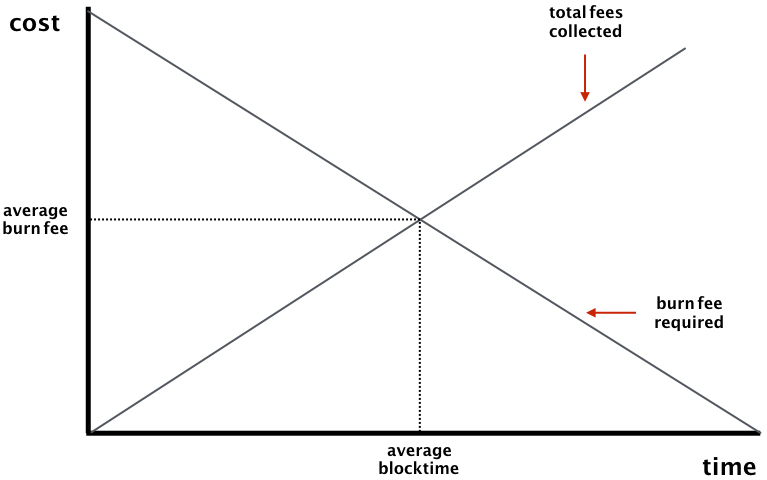
\includegraphics[width=.45\textwidth]{saito2.jpeg}
  \captionsetup{justification=raggedright,singlelinecheck=false,labelfont=bf}
  \captionof{figure}{The Burn Fee Curve}
  \label{fig:burnfee}
\end{minipage}
}

Saito derives routing work from the transaction fee embedded in every transaction. Using this measure of work to produce blocks makes attacking the network expensive, since making claims about time cost money. It can be seen from Figure 2 that it is impossible for attackers to produce blocks at a faster pace than the main chain unless they have access to a larger pool of transaction fees.

\makebox[0pt][l]{%
\begin{minipage}{\textwidth}
  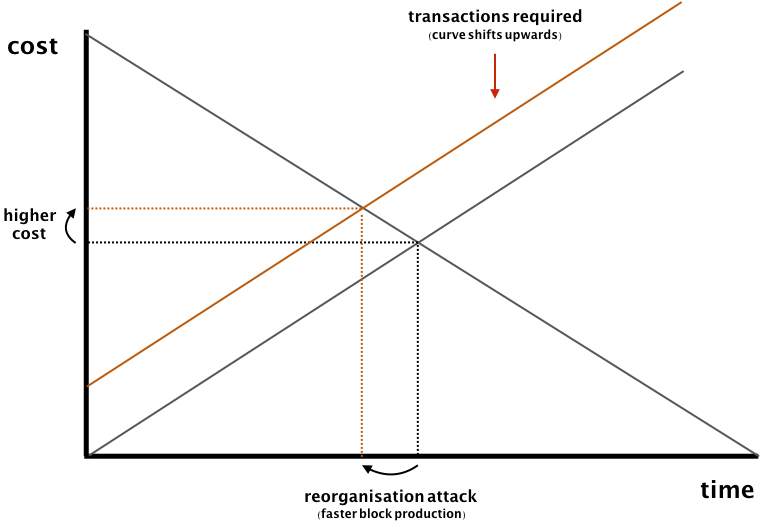
\includegraphics[width=.45\textwidth]{saito3.jpeg}
  \captionsetup{justification=raggedright,singlelinecheck=false,labelfont=bf}
  \captionof{figure}{Good Actor Burn Fee Costs... }
  \label{fig:burnfee}
\end{minipage}
}

To secure this mechanism, Saito has routing nodes cryptographically sign transactions as they propagate through the network. Consensus rules specify that the amount of "routing work" a transaction provides any node drops with the number of hops in its routing path, and that transactions provide no usable routing work to nodes that are not in their routing path. The work used to produce blocks is the efficient collection and sharing of inbound network fees.

As long as there is no payment for block production this system offers comparable security to Bitcoin: cost-of-attack can always be quantified and attackers must spend their own money to attack the chain. This allow users to wait however many confirmations are needed to meet their security requirements. As a bonus, the network can increase the amount of "routing work" needed for block production to keep blocktime constant as transaction volume grows, so that security scales with fee-volume.

The major problem with this approach lies in the consequences of requiring the network to burn capital to produce blocks:

\makebox[0pt][l]{%
\begin{minipage}{\textwidth}
  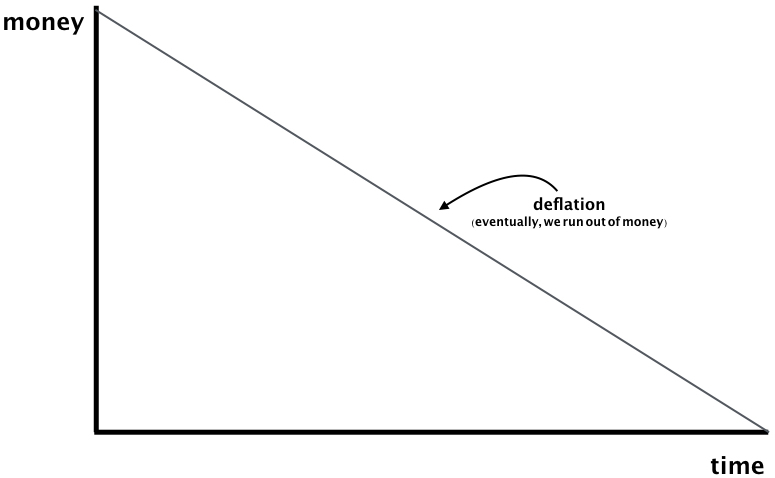
\includegraphics[width=.45\textwidth]{saito4.jpeg}
  \captionsetup{justification=raggedright,singlelinecheck=false,labelfont=bf}
  \captionof{figure}{Deflation of Burn Fee Over Time}
  \label{fig:burnfee}
\end{minipage}
}

Avoiding a deflationary crash requires us to inject tokens back into our network. But Saito cannot simply give the fees directly to block producers: that would allow attackers to use the income from one block to generate the routing work needed to produce the next. Dividing up the payment between different nodes is preferable, but as long as block-producers have any influence over who gets paid a savvy attacker can sybil the network or conduct grinding attacks that target the token-issuing mechanism.

Solving this problem requires inverting the classic proof-of-work solution. In Bitcoin, consensus rules make it expensive to produce blocks and fees are then handed to the block producer. This is meant to ensure block production is expensive but in reality guarantees there are always conditions under which attacks are profitable.\footnote[1]{Many core problems with the proof-of-work and proof-of-stake mechanisms stem from this decision. Leaving aside the fifty-one percent attack, note the way supply-side constraints in external markets (i.e. inelastic supply curve for hashpower or capital) are used to impose a "cost constraint" on attackers. Not only does this design remove any ability for the blockchain to regulate its own security, but the profits available in external markets necessarily and inevitably commoditize the work function and flatten the supply-curve for the work-factor in the external market.} In Saito the solution is the opposite. The first-order problem changes into securing the payment mechanism: ensuring that payments are proportional to work regardless of who produces blocks. The cost-of-attack that a mechanism with this property creates is then leveraged into being the cost of block production.

We call the mechanism that achieves this the "golden ticket" solution. This mechanism pays honest nodes for collecting fees regardless of who produces blocks. The trick is pulling this off in a way that ensures there is always a quantifiable cost to attacking the system. The practical solution is returning the transactions fees to the network through a process that cannot be gamed by any of the players in the network without spending far more money on the attack than they stand to benefit from collecting the payments. Implementation details are described in the next section.

4. THE GOLDEN TICKET

Whenever a node produces a block, it may collect the difference between the amount of "routing work" included in its block and the amount of routing work required for block production. No other payments are made.

Unlocking those payments requires the network to solve a computational puzzle we call the "golden ticket". This puzzle requires knowledge of the block hash to solve and cannot be calculated in advance. Miners on the network listen for blocks as they are produced and begin hashing in search of a solution. Should they find a transaction they propagate it back into the network as a normal fee-paying transaction.

Only one solution may be included in any block, and that solution must be included in the very next block to be considered valid. If these conditions are violated or if a "golden ticket" is not solved, the funds that were not paid out in the previous block are simply not allocated. They fall backwards into the blockchain and eventually fall off the chain, at which point the lost funds are recollected by the consensus layer and eventually redistributed as part of a future block reward. 

Should a solution be found in time, the unallocated fees are released to the network; split between the miner that found the solution and a random node in the peer-to-peer routing network. The lucky routing node is selected using a random variable sourced from the miner solution, with each routing node's chance of winning normalized to be proportional of the overall "routing work" it contributed to the block being solved.

As transactions are routed into the network, it can be seen that the total claims on payment embedded in them (sum of routing work available to all nodes in the routing path) grow while the amount of work available to produce a block (the amount of routing work available to specific nodes) shrinks. Attackers who use honest transactions to produce blocks put themselves on-the-hook for paying the difference.

We call the division of payment between miners and routers the "paysplit" of the network. It is set to 0.5 by default (half to miners, half to routers) but can be made adjustable as described in the section below. The golden ticket system can be visualized as follows:

\makebox[0pt][l]{%
\begin{minipage}{\textwidth}
  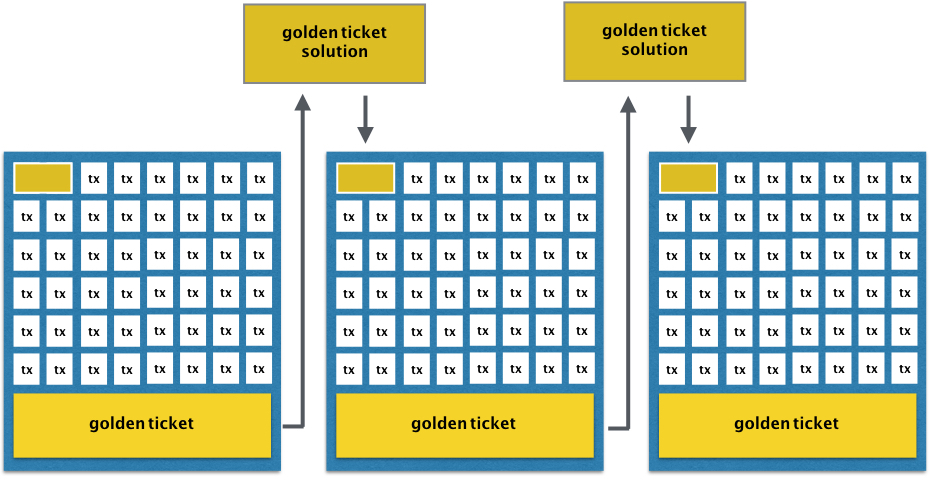
\includegraphics[width=.45\textwidth]{saito7.jpeg}
  \captionsetup{justification=raggedright,singlelinecheck=false,labelfont=bf}
  \captionof{figure}{The Golden Ticket System}
  \label{fig:burnfee}
\end{minipage}
}

This system has several major advantages over proof-of-work and proof-of-stake mechanisms. The most important is that Saito explicitly distributes fees to the nodes that service users, collect transactions and produce blocks, and does so in proportion to the amount of value that these actors provide to the overall network. Network nodes compete for access to lucrative inbound transaction flow, and will happily fund whatever development activities are needed to get users on the network. Of note, the services provided by edge nodes to attract Saito usage can include public-facing infrastructure needed by other blockchains.

This is a fundamental shift. Where other blockchains explicitly define which activities have value, Saito lets the users signal what services provide value through fee-pricing, while the network infers who deserves payment. Saito also incentivizes the efficient delivery of value to users. And by paying for value rather than a subset of network activities it provides the only way to guarantee that a self-sufficient network can remain open and economically independent at scale.

The Saito consensus mechanism is also "twice as secure" as its proof-of-work and proof-of-stake counterpoints. Honest nodes route transactions to block producers and earn fees in exchange. But attackers are thrown into a catch-22: they must not only spend the same amount of fees as the honest network to produce a competitive chain, but must also match 100 percent of mining output to find enough golden ticket solutions to recapture their funds.  Even if attackers successfully launch fee-recycling attacks, they must still spend 100 percent of their income on hashing.

The basic version of the Saito system achieves 100 percent fee-security, eliminating the fifty-one percent attack completely. Section 5 describes a modification to this mechanism that pushes security above 100 percent and guarantees that attackers will lose money in all circumstances. Regardless of which implementation is used, the economic problems created by mechanisms that rely on external supply-curves vanish: mining serves as a pure cost function instead of a difficulty function and the blockchain remains secure even if the supply curve for hashpower becomes perfectly flat.


5. ADVANCED SECURITY - POWSPLIT

It is possible to increase attack costs beyond 100 percent of available returns through a "powsplit" mechanism. Note that in the normal Saito implementation with a fixed paysplit of 0.5, the network auto-adjusts mining difficulty so that one solution is found per block, on average. Since miners cannot control the variance at which solutions are found, network difficulty may end up being lower on average than needed for optimal security.

A "powsplit" approach eliminates this problem by adjusting mining difficulty so that one solution is found every N blocks on average. When such a solution is included in the blockchain, if the previous block did not contain a golden ticket, the random variable used to pick the winning routing node is hashed again to select a winner from the unsolved block which preceded it or from a table of stakers as described below. An upper limit to backwards recursion may be applied for practical purposes, as the circular blockchain will recapture any funds that are not paid out.

To become stakers in the network, users broadcast a transaction containing a specially-formatted UTXO. These UTXO are added to a list of "pending stakers" on their inclusion in a block. Once the current staking table has been fully paid-out, all pending staking UTXO are moved into the current staking table. To avoid throttling attacks on the staking mechanism it is wise to not permit stakers to withdraw or spend staked UTXO until they have received payment. 

The percentage of network revenue allocated to staking nodes should be proportional to their share of the amount of fees paid into the treasury by the staking mechanism during the previous round. Limits may be put on the size of the staking pool to induce competition between stakers if desirable or prevent users from spamming the staking mechanism in the hope of dissuading honest stakers from participating. In normal situations the looping blockchain and ATR mechanism will prevent stakers from launching spam attacks as multiple UTXO will all pay rebroadcast fees.

To ensure the system works, block producers who rebroadcast UTXO must now indicate in their ATR transactions whether the specific outputs are active in the current or pending staking pool. A hash representation of the state of the staking table may be included in every block in the form of a commitment to allow nodes to verify the accuracy of the staking table, but the ATR rebroadcast mechanism will theoretically allow all nodes to reconstruct the state of the staking pool within one epoch at most.

Mining difficulty can be adjusted upwards if two blocks containing golden tickets are found in a row and downwards if two blocks without golden tickets are found consecutively. A similar punitive cost can throttle the staking payout if two blocks without golden tickets are found in a row (an ever-increasing amount of the staking revenue is withheld). We encourage those interested in the underlying mathematics to consult our papers on the topic. The cost of attacking a Saito network using this mechanism rises significantly above 100 percent. 


6. ADVANCED SECURITY - PAYSPLIT

There are several modifications to the paysplit mechanism that can be used to increase attack costs. While the version of Saito being launched for production does not include this mechanism, it is possible to add a dynamic voting system to Saito that can allow paysplit to float dynamically. This section describes a theoretical improvement that allows for a floating paysplit that will work under certain assumptions about the rationality of the network.

An implementation of this system modifies blocks so that they include a vote to increase, decrease or hold constant the paysplit of the network. Golden ticket solutions may be then modified so that they contain similar vote on the difficulty of the golden-ticket production function. The consensus variables of the network are updated when and only when golden tickets are solved and included in the blockchain.

Adjusting paysplit like this can change the distribution of fees between routing nodes and miners in real-time. This allows the network to reach an optimal equilibrium rather than an arbitrary one. To prevent this equilibrium from reflecting only the preferences of the routing and mining nodes, we recommend letting the users on the network tag their transactions with an optimal paysplit vote as well: should a user-originated transaction contain such a vote, it may only be included in a block that votes in the same direction. Users who take sides in the ongoing struggle between routers and miners thus sacrifice the reliability and speed of transaction confirmation, but gain marginal influence over how the network allocates fees. Users making votes are also withholding their fees from nodes voting differently to themselves.

Under conditions where network participants exhibit bounded rationality, this mechanism pushes paysplit to the point where the security provided is optimal for all participants given the cost of additional fee collection. De Toqueville compacts secure the equilibrium: any two players in the tripartite network structure (routers, miners, users) may team-up to shift the paysplit back to the desired ideal. While we leave research into this mechanism for the future, a useful thought experiment is exploring how the security of this three-player system degrades to only bitcoin-class security as the paysplit approaches extreme values.


7. ADDITIONAL NOTES ON NETWORK SECURITY

Saito's design solves several long-standing problems of note. Hoarding attacks are minimized because nodes that participate in transaction routing maximize revenue by finding the most efficient routing path into the network. Competition encourages the sharing of fees rather than the hoarding of fees. The availability of routing information in blocks also allows participants to check that their peers are faithfully propagating their transactions instead of hoarding them.

Because adding hops to any routing path necessarily reduces the profitability of routing for every node in the path, sybil attacks are also eliminated. Blocks provide the information needed for participants to identify and eliminate sybils in their peer-to-peer networks. And evolutionary pressures ensures that they will purge them: weaker nodes which permit themselves to be sybilled will find themselves driven out of the network by competitive pressures over time.

The routing network also serves a unique defensive mechanism. Routing nodes in Saito can increase the cost of attack in real-time by refusing to route transactions to attackers, forcing an increased reliance by the attacker on their own wallet to fund block production. This mechanism also defends Saito against subtle attacks like monetizing transaction flows and closed-access routing.

As a final observation, we note that the "scalability trilemma" often championed as a fundamental law of blockchain does not exist in the Saito design. There are many obvious configurations of the network in which redirecting fees from miners to routing nodes can simultaneously increase the throughput, decentralization and security of the network simultaneously.


8. SUMMARY

The fundamental problems affecting blockchain scaling are economic. Saito fixes these issues, allowing us to build a massively-scalable blockchain which achieves scalability by ensuring that payments flow to the nodes that spend money on network infrastructure.

Those who pour over the technical details of the Saito network will find embedded in it at least seven major innovations in blockchain technology: automatic transaction rebroadcasting, the burn fee, the golden ticket system, paysplit and powsplit, N-block golden tickets, a secure multi-party voting mechanism, and the chain of cryptographic signatures that permits the blockchain to identify and reward productive nodes in the routing network.

Patent protection has been secured on these techniques and we welcome contact from other blockchain projects looking to incorporate one or several of these methods in their own networks. We also encourage readers to visit our website (https://saito.io) which includes an interface for the working network, a roadmap outlining future development plans, and tutorials that can help anyone get started building Saito applications \textbf{today}.

\end{multicols}
\end{document}
